\documentclass[../main.tex]{subfiles}

\begin{document}
	\section{Gradino}
		\begin{figure}[H]
			\centering
			\begin{subfigure}{0.4\textwidth}
				\[
					\gr = 
					\begin{cases}
						0 \quad t<0
						\\
						1 \quad t \geq 0
					\end{cases}
				\]
			\end{subfigure}
			\begin{subfigure}{0.4\textwidth}
				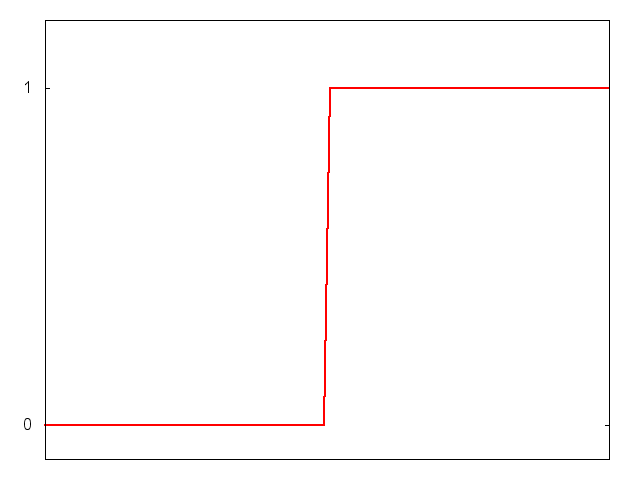
\includegraphics[width=.5\textwidth]{funzioni_generalizzate/gradino}
			\end{subfigure}
		\end{figure}
		Presenta una discontinuità in $ t=0 $.
		
	\section{Rampa}
		\begin{figure}[H]
			\centering
			\begin{subfigure}{0.4\textwidth}
				\[
					ram(t)= t \cdot \gr =
					\begin{cases}
						0 \quad t<0
						\\
						t \quad t \geq 0			
					\end{cases}
				\]
			\end{subfigure}
			\begin{subfigure}{0.4\textwidth}
				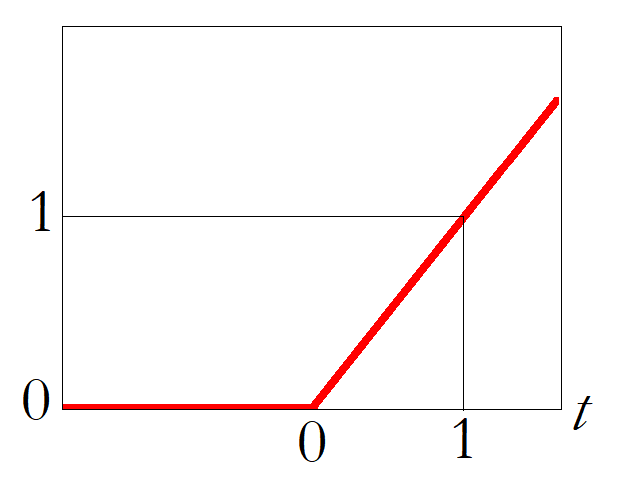
\includegraphics[width=.5\textwidth]{funzioni_generalizzate/rampa}
			\end{subfigure}
		\end{figure}
		In $ t=0 $ \'e continua, ma presenta una discontinuit\'a di prima specie nella derivata.
		
	\section{Parabola}
		\begin{figure}[H]
			\centering
			\begin{subfigure}{0.4\textwidth}
				\[
					par(t) = 
					\begin{cases}
						0 \quad &t<0
						\\
						\frac{t^2}{2} \quad &t\geq 0
					\end{cases}
				\]
			\end{subfigure}
			\begin{subfigure}{0.4\textwidth}
				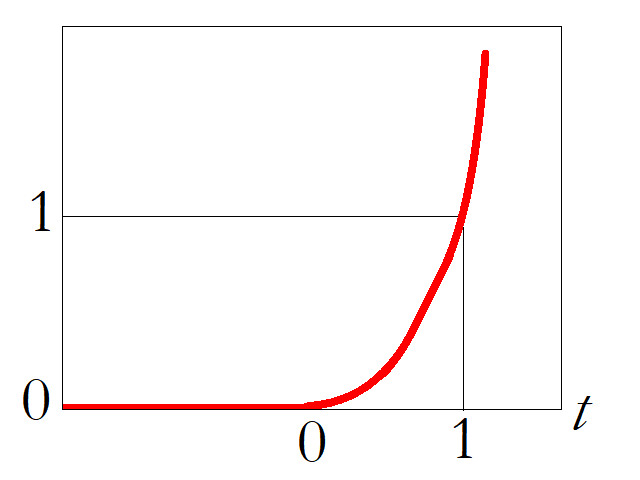
\includegraphics[width=.5\textwidth]{funzioni_generalizzate/parabola}
			\end{subfigure}
		\end{figure}
		Risulta continua e con derivata continua anche in $ t=0 $.	
		
	\section{Polinomio di grado n}
		\[
			pol(t)=\frac{t^n}{n} \cdot \gr =
			\begin{cases}
				0 \quad &t<0
				\\
				\frac{t^n}{n} \quad &t\geq 0
			\end{cases}
		\]
		
	\section{Derivate e integrali delle funzioni generalizzate}
		\begin{align*}
			&ram(t) = \int_{- \infty}^{t} \gr[\tau] \mathrm{d}\tau &&\der{}{t} ram(t) = \gr
			\\
			&par(t) = \int_{- \infty}^{t} ram(\tau) \mathrm{d} \tau &&\der{}{t} par(t) = ram(t)	
		\end{align*}
		
	\section{Impulso}
		Introduco la funzione $ \textbf{1}_{\Delta}(t) $ definita come:
		\[
			\int_{- \infty}^{t} \der{}{t}1_{\Delta}(t) \mathrm{d}\tau=
			\begin{cases}
				1 \quad t>\Delta\\
				0 \quad t<0
			\end{cases}
		\]
		Non consideriamo il caso in cui $ 0<t<\Delta $.\\
		\linebreak
		Definisco $ \delta(t) $ la funzione $ \der{}{t}1_{\Delta}(t) $ quando $ \Delta \longrightarrow 0 $. Valgono dunque le seguenti relazioni: 
		\begin{figure}[H]
			\centering
			\begin{subfigure}{0.5\textwidth}
				\[
					\int_{-t}^{t} \delta(\tau) \mathrm{d}\tau =1 \quad \forall t>0, \qquad \der{}{t} \gr = \delta(t)
				\]
			\end{subfigure}
			\begin{subfigure}{0.4\textwidth}
				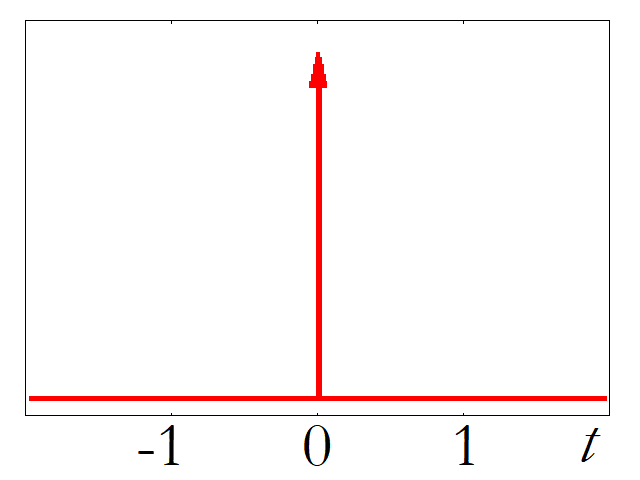
\includegraphics[width=.5\textwidth]{funzioni_generalizzate/impulso}
			\end{subfigure}
		\end{figure}
		L'impulso \'e caratterizzato dal valore della sua area, determinato dal coefficiente della funzione.\\
		\linebreak
		L'impulso torna utile quando bisogna effettuare il \textbf{campionamento} di una funzione, cio\'e determinare il valore della funzione nel punto in cui viene applicato l'impulso.
		\begin{align*}
			f(t)\ \delta(t) &= f(0)\ \delta(t)\\
			f(t)\ \delta(t - T) &= f(T)\ \delta(t - T)   
		\end{align*}
		
	\section{Doppietto}
		Derivando ulteriormente $ \der{}{t}1_{\Delta}(t) $ in un intorno $ I(0) $ e in $ I(\Delta) $ si ottengo due impulsi unitari: il primo centrato nell'origine, mentre il secondo centrato in $ \Delta $ e negativo.\\
		Per $ \Delta \longrightarrow 0 $ si ottiene:
		\begin{figure}[H]
			\centering
			\begin{subfigure}{0.5\textwidth}
				\[
					\der{}{t} \delta(t) = \dot{\delta}(t)
				\]
			\end{subfigure}
			\begin{subfigure}{0.4\textwidth}
				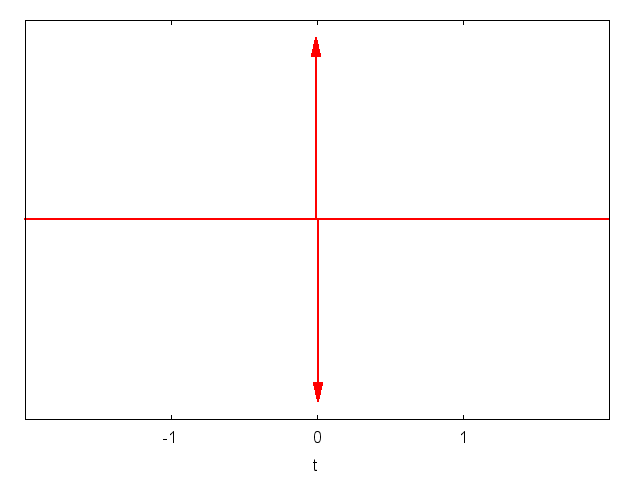
\includegraphics[width=.5\textwidth]{funzioni_generalizzate/doppietto}
			\end{subfigure}
		\end{figure}
		
	\section{Riepilogo}
		\[
			par(t) \quad \stackrel[\int_{-\infty}^{t}]{\der{}{t}}{\rightleftharpoons} 
			\quad ram(t) \quad
			\stackrel[\int_{-\infty}^{t}]{\der{}{t}}{\rightleftharpoons}
			\quad \gr \quad
			\stackrel[\int_{-\infty}^{t}]{\der{}{t}}{\rightleftharpoons}
			\quad \delta (t) \quad
			\stackrel[\int_{-\infty}^{t}]{\der{}{t}}{\rightleftharpoons}
			\quad \dot{\delta}(t) \quad
		\]
		
	\section{Trasformazioni delle funzioni}
	
	\subsection{Traslazione}
		\begin{figure}[H]
			\centering
			\begin{subfigure}{0.5\textwidth}
				\[
					f(t) = f(t - T)
				\]
				\begin{itemize}
					\item $ T>0 $: ritardo, la funzione \'e traslata verso dx di t
					\item $ T<0 $: anticipo, la funzione \'e traslata verso sx di t 	
				\end{itemize}
			\end{subfigure}
			\begin{subfigure}{0.4\textwidth}
				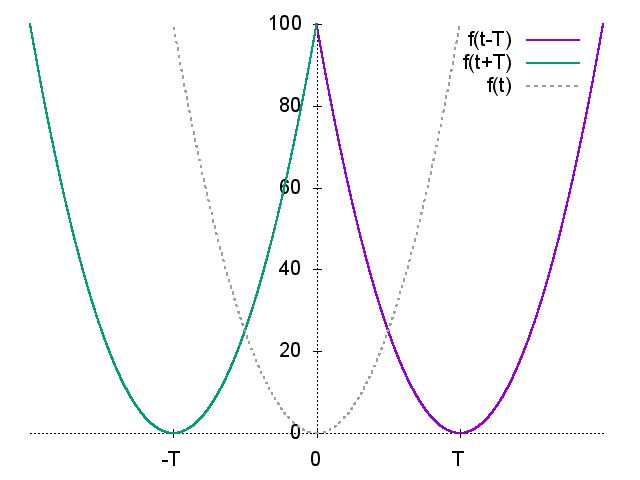
\includegraphics[width=\textwidth]{funzioni_generalizzate/traslazione}
			\end{subfigure}
		\end{figure}
		
	\subsection{Scalamento}
		\begin{figure}[H]
			\centering
			\begin{subfigure}{0.5\textwidth}
				\[
					f(t) = f(t \cdot \alpha)
				\]
				\begin{itemize}
					\item $ 0 < \alpha < 1 $: la funzione si estende di un fattore t
					\item $ \alpha > 1 $: la funzione viene compressa di un fattore t  
				\end{itemize}
			\end{subfigure}
			\begin{subfigure}{0.4\textwidth}
				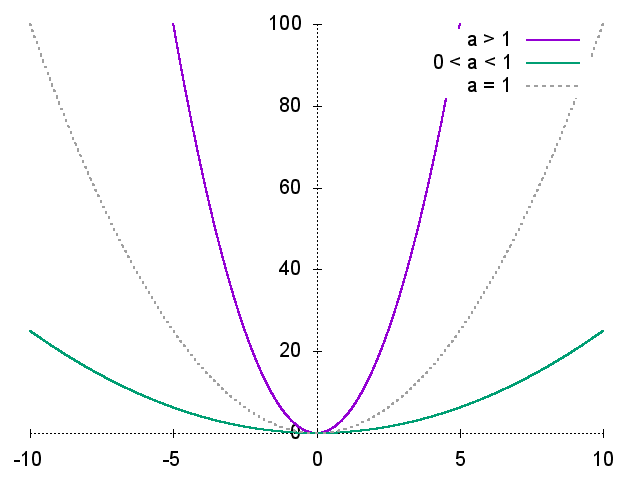
\includegraphics[width=\textwidth]{funzioni_generalizzate/scalamento}
			\end{subfigure}
		\end{figure}
		
	\subsection{Simmetrie}
		\begin{itemize}
			\item $ f(t) = f(-t) $: simmetrica rispetto l'asse delle y
			\item $ f(t) = -f(t) $: simmetrica rispetto l'asse delle x  	
		\end{itemize}
		\begin{figure}[H]
			\centering
			\begin{subfigure}{0.45\textwidth}
				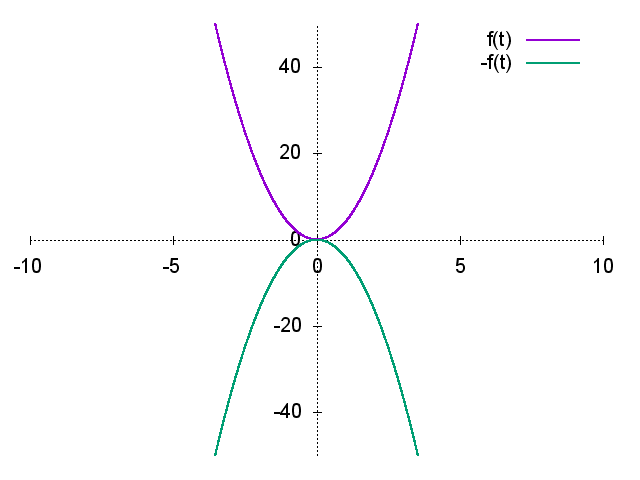
\includegraphics[width=\textwidth]{funzioni_generalizzate/simmetria_x}
				\caption{simmetria rispetto l'asse x}
			\end{subfigure}
			\begin{subfigure}{0.45\textwidth}
				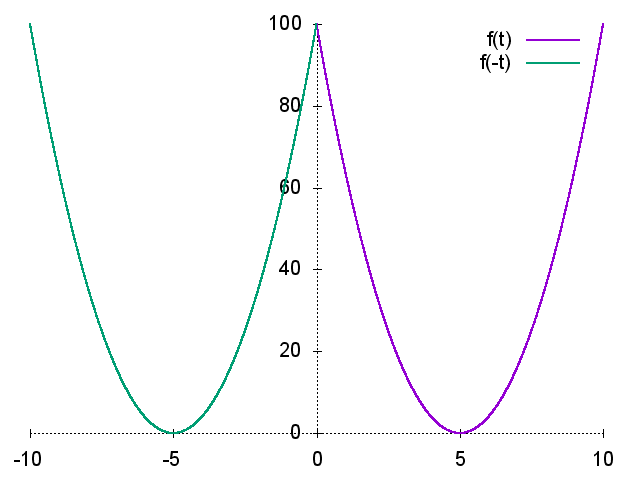
\includegraphics[width=\textwidth]{funzioni_generalizzate/simmetria_y}
				\caption{simmetria rispetto l'asse y}
			\end{subfigure}
		\end{figure}
		
	\section{Rettangolo}
		\begin{figure}[H]
			\centering
			\begin{subfigure}{0.5\textwidth}
				\[
					R_{t_{1},t_{2}}(t) = \gr[t - t_{1}] - \gr[t - t_{2}]
				\]
			\end{subfigure}
			\begin{subfigure}{0.4\textwidth}
				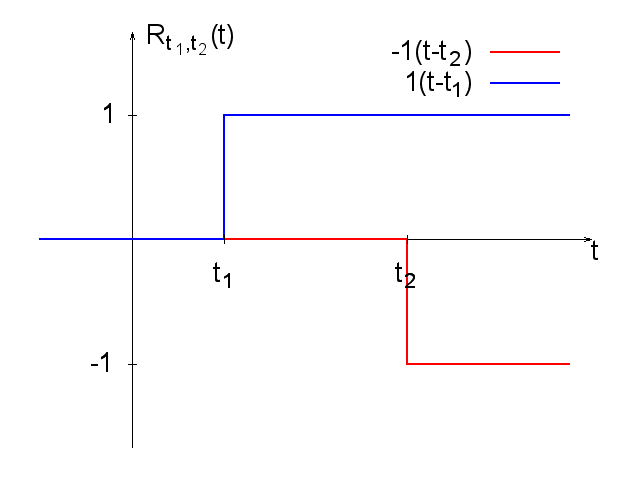
\includegraphics[width=\textwidth]{funzioni_generalizzate/rettangolo}
			\end{subfigure}
		\end{figure}
		
		\begin{mdframed}[style=Exercise]
			\begin{Exercise}[title={Derivata di una funzione definita a tratti}, difficulty=3]
				Dividiamo il grafico \ref{fig:grafico_f} in sezioni e per ognuna scriviamo la funzione \textit{finestrata} (cio\'e moltiplicata per un rettangolo di base pari alla larghezza della sezione):
				\begin{figure}[H]
					\centering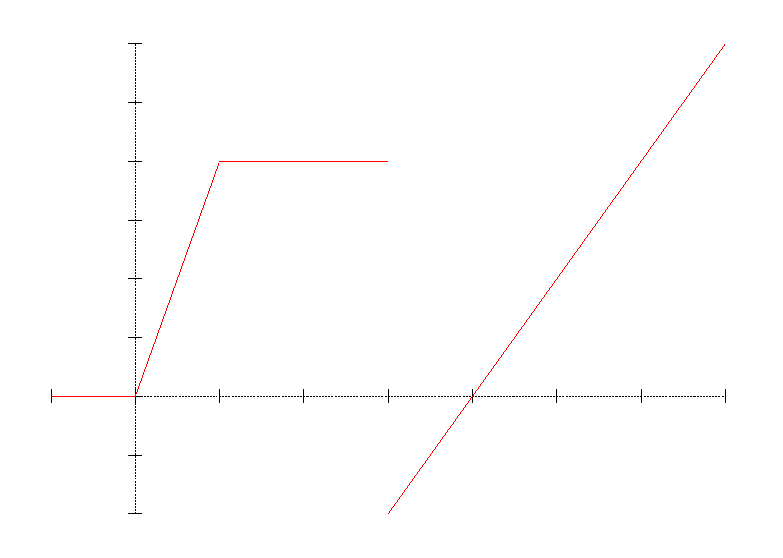
\includegraphics[width=.4\textwidth]{funzioni_generalizzate/esercizi/derivata_funzione_def_tratti}
					\caption{Grafico di $ f(t) $}
					\label{fig:grafico_f}
				\end{figure}
				\[
					f(t) = 2t \cdot R_{0,1}(t) + 2 \cdot R_{1,3}(t) + (t-4) \cdot R_{3,\infty}(t)
				\]
				Riscriviamo i rettangoli attraverso i gradini:
				\[
					\begin{aligned}
						f(t) &= 2t \cdot \big[ \gr[t-0] - \gr[t-1] \big] + 2\ \big[\gr[t-1] - \gr[t-3]\big] + (t-4)\ \big[\gr[t-3] - \underbrace{\gr[t - \infty]}_{0} \big] =
						\\
						&= 2t \cdot \gr[t] + (-2t+2) \cdot \gr[t-1] + (-2+t-4) \cdot \gr[t-3] =
						\\
						&= 2t \cdot \gr[t] - 2(t-1) \cdot \gr[t-1] + (t-6) \cdot \gr[t-3]
					\end{aligned}
				\]
				Quindi si pu\'o continuare in due modi equivalenti:
				\begin{enumerate}
					\item 
						si riconducono le funzioni a funzioni generalizzate e si deriva:
						\begin{align}
							\intertext{se sostiutiamo: $ (t-6) \cdot \gr[t-3] = (t-3) \cdot \gr[t-3] - 3 \cdot \gr[t-3] = ram(t-3) - 3 \cdot \gr[t-3] $}
							f(t) &= 2 \cdot ram(t) &&- 2 \cdot ram(t-1) &&+ram(t-3) &&- 3 \cdot \gr[t-3] \nonumber\\
							\dot{f(t)} &= 2 \cdot \textbf{1}(t) &&- 2 \cdot \gr[t-1] &&+ \gr[t-3] && - 3 \cdot \delta(t-3)
							\label{derivata_es11.2}
						\end{align}
					\item 
						si usano le derivate del prodotto:
						\[
							\dot{f(t)} = \big[ 2 \cdot \gr[t] + 2t \cdot \delta(t) \big]\ -\ 2 \cdot \gr[t-1]\ -\ 2 \cdot (t-1) \cdot \delta(t-1)\ +\ \gr[t-3]\ +\ (t-6) \cdot \delta(t-3)
						\]
						Attraverso il campionamento si ha che:
						\begin{itemize}
							\item 
								$ t \cdot \delta(t) = 0 $: campionamento in zero della retta passante per l'origine
							\item
								$ (t-1) \cdot \delta(t-1) = 0$: analogo al punto precedente
							\item
								$ (t-6) \cdot \delta(t-3) = - 3 \cdot \delta(t-3) $: la retta $ y=t-6 $ calcolata in $ t=3 $ vale -3. 
						\end{itemize}
						Dopo queste semplificazioni si ottiene l'espressione \ref{derivata_es11.2}.
				\end{enumerate}
			\end{Exercise}
		\end{mdframed}
\end{document}